\documentclass[conference]{IEEEtran}

\usepackage{cite}
\usepackage{amsmath,amssymb,amsfonts}
\usepackage{algpseudocode}
\usepackage{algorithm}
\usepackage{graphicx}
\usepackage{textcomp}
\usepackage{xcolor}
\def\BibTeX{{\rm B\kern-.05em{\sc i\kern-.025em b}\kern-.08em
    T\kern-.1667em\lower.7ex\hbox{E}\kern-.125emX}}
\begin{document}

\title{Forest Cover Classification\\

}

\author{\IEEEauthorblockN{David Nicolay}
\IEEEauthorblockA{\textit{Department of Computer Science} \\
\textit{Stellenbosch University}\\
Stellenbosch, South Africa \\
26296918@sun.ac.za}
}

\maketitle

\begin{abstract}
This document is a model and instructions for \LaTeX.
This and the IEEEtran.cls file define the components of your paper [title, text, heads, etc.]. *CRITICAL: Do Not Use Symbols, Special Characters, Footnotes, 
or Math in Paper Title or Abstract.
\end{abstract}

\begin{IEEEkeywords}
component, formatting, style, styling, insert.
\end{IEEEkeywords}

\section{Introduction}
introooo TODO remove
``Fig.~\ref{fig}'', even at the beginning of a sentence.

\begin{table}[htbp]
\caption{Table Type Styles}
\begin{center}
\begin{tabular}{|c|c|c|c|}
\hline
\textbf{Table}&\multicolumn{3}{|c|}{\textbf{Table Column Head}} \\
\cline{2-4} 
\textbf{Head} & \textbf{\textit{Table column subhead}}& \textbf{\textit{Subhead}}& \textbf{\textit{Subhead}} \\
\hline
copy& More table copy$^{\mathrm{a}}$& &  \\
\hline
\multicolumn{4}{l}{$^{\mathrm{a}}$Sample of a Table footnote.}
\end{tabular}
\label{tab1}
\end{center}
\end{table}

\begin{figure}[htbp]
\centerline{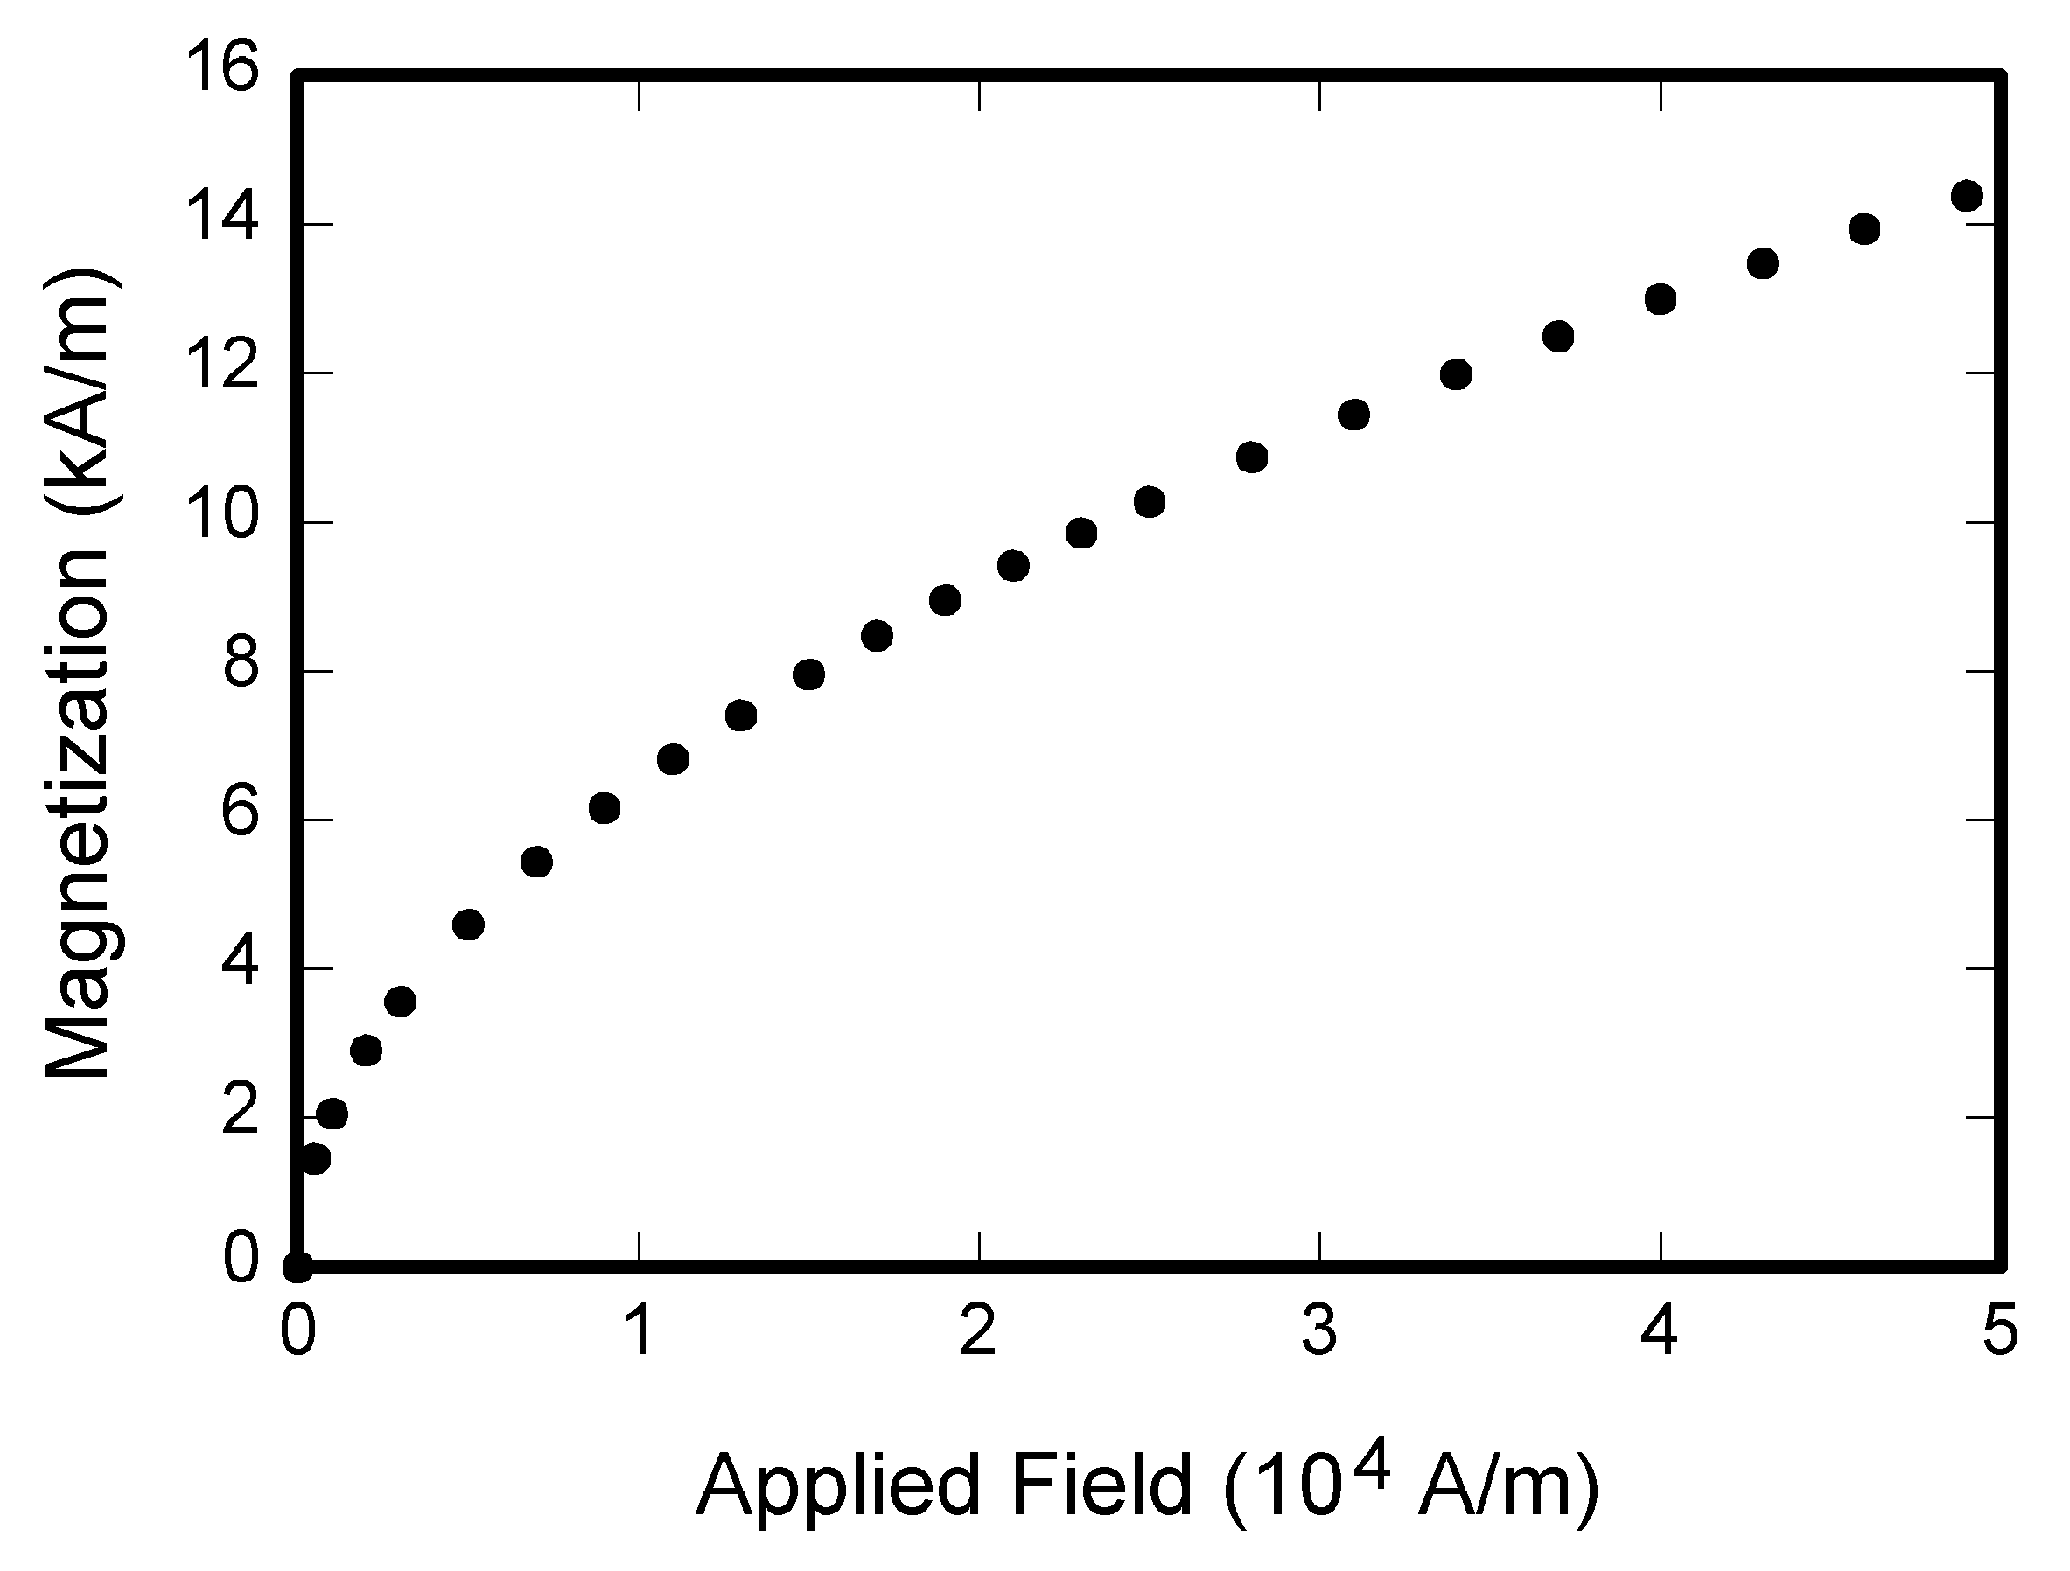
\includegraphics{fig1.png}}
\caption{Example of a figure caption.}
\label{fig}
\end{figure}

Figure Labels: Use 8 point Times New Roman for Figure labels. Use words 
rather than symbols or abbreviations when writing Figure axis labels to 
avoid confusing the reader. As an example, write the quantity 
``Magnetization'', or ``Magnetization, M'', not just ``M''. If including 
units in the label, present them within parentheses. Do not label axes only 
with units. In the example, write ``Magnetization (A/m)'' or ``Magnetization 
\{A[m(1)]\}'', not just ``A/m''. Do not label axes with a ratio of 
quantities and units. For example, write ``Temperature (K)'', not 
``Temperature/K''.

\section{Introduction}
\section{Background}

\subsection{k-nearest Neighbours (kNN)}
The nearest neighbour algorithm is an example of instance-based learning where the prediction for an instance is made by comparing the instance to similar training instances. This is a lazy learning approach since we delay processing training data until prediction is needed. Since kNN is also similarity-based, it is non-parametric, which means that it does not learn a mapping from the input space to the output space.

The k-nearest neighbour algorithm is presented in Algorithm~\ref{alg:knn} which explains that we calculate the distance from each data point in our training dataset to the distance. From there, we choose the closed \textit{k} observations and perform inference. In a classification context we may perform majority voting to determine the class, in a regression context we use the mean or median of the \textit{k} nearest observations.

In order to use the algorithm we need to define a value of \textit{k} which decides the number of nearest neighbour instances to consider when predicting. Choosing a value a low value for \textit{k} results in a high variance, but low bias leading to an unstable model which tends to overfit. Choosing a large value for \textit{k} results in a smaller variance, but high bias, leading to a more stable model which tending to underfit. Measures such as \textit{k}-fold cross validation assist in the selection of a value of \textit{k}.

\begin{algorithm}[htbp]
\caption{k-Nearest Neighbors Algorithm}
\label{alg:knn}
\begin{algorithmic}
\Function{kNN}{$D, x, k$}
\ForAll{$x' \in D$}
\State $d = \text{distance}(x, x')$
\EndFor
\State sort($d$)
\State $S = $ set of $k$ patterns in $D$ closest to $x$
\State \Return class as majority class in $S$
\EndFunction
\end{algorithmic}
\end{algorithm}
\noindent
\textbf{Notation:} $D$ denotes the training dataset, $x$ is the query instance, $k$ is the number of nearest neighbours, and $\text{distance}(\cdot)$ is a distance metric (e.g., Euclidean distance).


\subsection{Classification Trees}
Classification trees represent a fundamental approach in supervised machine learning for predictive modelling, where the learned model forms a hierarchical tree structure with non-terminal nodes representing decisions on descriptive features and terminal leaf nodes representing target feature predictions \cite{quinlan1993c45}. A classification tree is a type of decision tree where leaf nodes represent different discrete classes.

\subsection{Expectations With Respect to Data Quality Issues}

\section{Methodology}
\section{Empirical Procedure}
\section{Research Results}
\section{Conclusion}
\section*{References}

Please number citations consecutively within brackets \cite{eason1955}. The 
sentence punctuation follows the bracket \cite{maxwell1892}. Refer simply to the reference 
number, as in \cite{jacobs1963}---do not use ``Ref. \cite{jacobs1963}'' or ``reference \cite{jacobs1963}'' except at 
the beginning of a sentence: ``Reference \cite{jacobs1963} was the first $\ldots$''

Number footnotes separately in superscripts. Place the actual footnote at 
the bottom of the column in which it was cited. Do not put footnotes in the 
abstract or reference list. Use letters for table footnotes.

Unless there are six authors or more give all authors' names; do not use 
``et al.''. Papers that have not been published, even if they have been 
submitted for publication, should be cited as ``unpublished'' \cite{elissa}. Papers 
that have been accepted for publication should be cited as ``in press'' \cite{nicole}. 
Capitalize only the first word in a paper title, except for proper nouns and 
element symbols.

For papers published in translation journals, please give the English 
citation first, followed by the original foreign-language citation \cite{yorozu1987}.

\bibliographystyle{IEEEtran}
\bibliography{references}

\end{document}
